\documentclass[11pt]{article}

\usepackage[utf8]{inputenc}
\usepackage{amsmath,amssymb,graphicx,booktabs,geometry,caption}
\usepackage{float}
\usepackage{listings}
\usepackage{xcolor}
\geometry{margin=1in}
\setlength{\parskip}{0.6em}
\setlength{\parindent}{0pt}

\lstset{
  inputencoding=utf8,
  extendedchars=true,
  basicstyle=\ttfamily\small,
  backgroundcolor=\color{gray!5},
  frame=single,
  breaklines=true,
  showstringspaces=false,
  keywordstyle=\color{blue},
  commentstyle=\color{gray},
  literate=
    {–}{{-}}1
    {—}{{-}}1
    {“}{{"}}1
    {”}{{"}}1
    {‘}{{'}}1
    {’}{{'}}1
    {…}{{...}}1
    {‐}{{-}}1
}

\title{Value at Risk and Expected Shortfall for Microsoft (MSFT)}
\author{Haesoo Pyun}
\date{}

\begin{document}
\maketitle

\section*{Introduction}
This report estimates one-day Value at Risk (VaR) and Expected Shortfall (ES) for Microsoft (MSFT) using the variance-covariance (VCV, normal) and historical simulation (HS) approaches. We analyse unconditional risk over the sample and conditional risk on 22~Aug~2025 using EWMA(0.94) volatility. The objective is to compare parametric and non-parametric estimates and show how time-varying volatility affects tail risk.

\section*{Method}
Let $r_t=\ln(P_t/P_{t-1})$. Under VCV (normal):
\[
\mathrm{VaR}_{\mathrm{VCV}} = -(\mu + \sigma q_\alpha),\qquad
\mathrm{ES}_{\mathrm{VCV}} = \frac{\sigma \phi(q_\alpha)}{\alpha},
\]
where $q_\alpha=\Phi^{-1}(\alpha)$ and $\phi(\cdot)$, $\Phi(\cdot)$ are the standard normal pdf and cdf.
For HS, $\mathrm{VaR}_{\mathrm{HS}}$ is the empirical $\alpha$-quantile and
\[
\mathrm{ES}_{\mathrm{HS}} = -\mathbb{E}[r_t \mid r_t \le -\mathrm{VaR}_{\mathrm{HS}}].
\]
Conditional volatility is EWMA(0.94): $\sigma_t^2=0.94\,\sigma_{t-1}^2+0.06\,r_{t-1}^2$.
Conditional VaR/ES at 22~Aug~2025 use $\sigma_T$ and the last 500 standardised returns.

\newpage
\section*{Results}
Table~\ref{tab:uncond} reports unconditional one-day VaR and ES for MSFT (daily, simple returns).
Risk grows monotonically with confidence. At 95\%, VCV VaR is 2.8769\% versus HS VaR of 2.6599\%. By 99\%, HS VaR (4.7845\%) exceeds VCV (4.09297\%), indicating a heavier extreme tail than the normal model. ES is consistently higher than VaR, and HS ES exceeds VCV ES across the grid.

\begin{table}[H]
\centering
\caption{Unconditional VaR and ES for MSFT (daily, simple returns)}
\label{tab:uncond}
\begin{tabular}{lcccc}
\toprule
Confidence & VaR (VCV) & ES (VCV) & VaR (HS) & ES (HS) \\
\midrule
90\% & 0.02234434 & 0.03072451 & 0.01809384 & 0.03170036 \\
91\% & 0.02338856 & 0.03160211 & 0.01936284 & 0.03313952 \\
92\% & 0.02452416 & 0.03256291 & 0.02075080 & 0.03480561 \\
93\% & 0.02577428 & 0.03362793 & 0.02237411 & 0.03669804 \\
94\% & 0.02717227 & 0.03482760 & 0.02455012 & 0.03890583 \\
95\% & 0.02876900 & 0.03620839 & 0.02659900 & 0.04164943 \\
96\% & 0.03064813 & 0.03784694 & 0.02943578 & 0.04501418 \\
97\% & 0.03296299 & 0.03988841 & 0.03343547 & 0.04966853 \\
98\% & 0.03604824 & 0.04262834 & 0.03887568 & 0.05671192 \\
99\% & 0.04092970 & 0.04702989 & 0.04784450 & 0.07104446 \\
\bottomrule
\end{tabular}
\end{table}

Figure~\ref{fig:uncond} illustrates MSFT's daily simple returns with the 95\% and 99\% unconditional VaR lines.
The series exhibits clear volatility clustering: periods of calm with small fluctuations are followed by bursts of large losses and gains, especially during financial stress episodes such as 2008--2009 and 2020.
The blue (HS) VaR lines lie consistently below the red (VCV) lines, implying that the historical distribution assigns greater probability to extreme losses than the normal model.
Several return spikes exceed even the 99\% VaR boundaries, demonstrating that both methods occasionally underpredict tail risk during turbulent periods.
Overall, the figure visually confirms leptokurtosis and time-varying volatility in MSFT returns, validating the need for a conditional (EWMA) framework.

\begin{figure}[H]
\centering
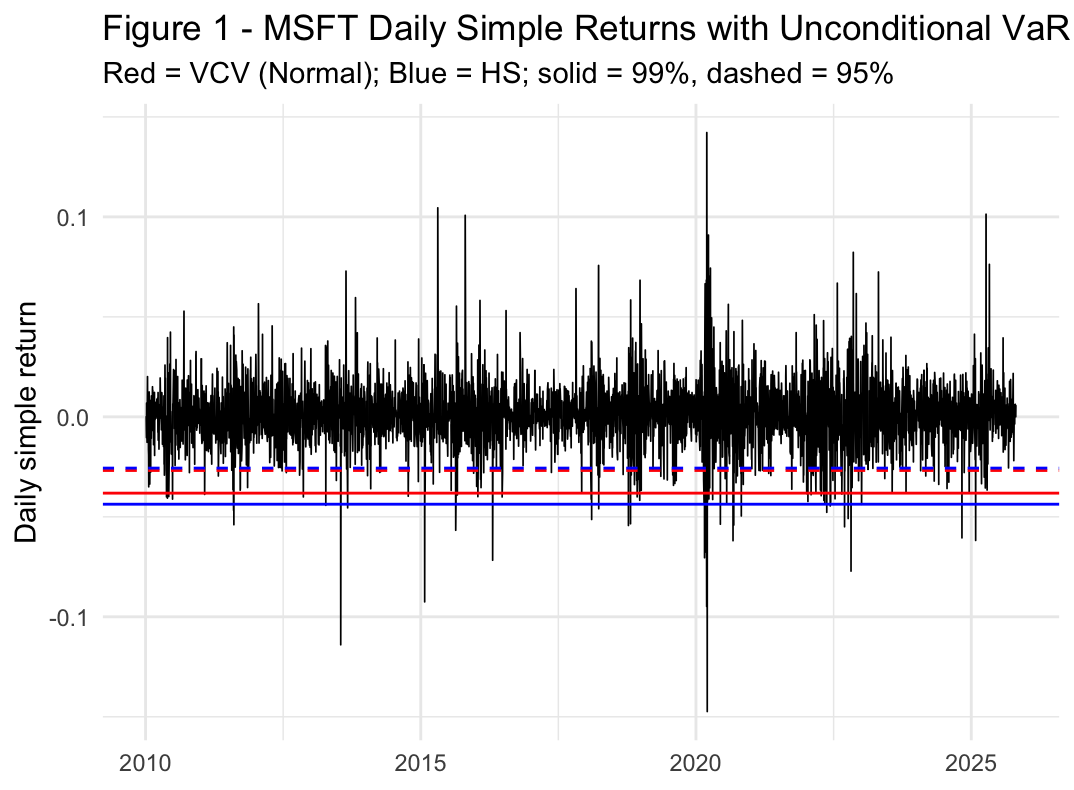
\includegraphics[width=0.9\textwidth]{figure_1.png}
\caption{MSFT daily returns with unconditional VaR lines (Red = VCV, Blue = HS; solid = 99\%, dashed = 95\%).}
\label{fig:uncond}
\end{figure}

Table~\ref{tab:cond} shows conditional one-day VaR and ES on 22~Aug~2025 using EWMA(0.94).
These are below the unconditional figures at each confidence level, implying relatively subdued volatility at that date.
At 95\%, conditional VCV VaR and ES are 1.8697\% and 2.3502\%, while HS VaR and ES are 1.9915\% and 3.0188\%, respectively.
HS estimates exceed VCV (especially ES), consistent with heavier empirical tails.

\begin{table}[H]
\centering
\caption{Conditional VaR and ES for MSFT on 22 Aug 2025 (EWMA 0.94; daily, simple returns)}
\label{tab:cond} % ← label immediately after caption
\begin{tabular}{lcccc}
\toprule
Confidence & VaR (VCV) & ES (VCV) & VaR (HS) & ES (HS) \\
\midrule
90\% & 0.01453720 & 0.01996084 & 0.01399364 & 0.02347603 \\
91\% & 0.01521386 & 0.02052794 & 0.01586047 & 0.02447826 \\
92\% & 0.01594946 & 0.02114860 & 0.01645833 & 0.02552838 \\
93\% & 0.01675891 & 0.02183636 & 0.01726701 & 0.02676907 \\
94\% & 0.01766371 & 0.02261078 & 0.01834187 & 0.02829910 \\
95\% & 0.01869661 & 0.02350173 & 0.01991488 & 0.03018831 \\
96\% & 0.01991148 & 0.02455846 & 0.02245770 & 0.03199048 \\
97\% & 0.02140699 & 0.02587145 & 0.02509336 & 0.03463847 \\
98\% & 0.02339841 & 0.02763877 & 0.02723740 & 0.03873643 \\
99\% & 0.02654502 & 0.03047004 & 0.03492866 & 0.04611230 \\
\bottomrule
\end{tabular}
\end{table}

\section*{Conclusion}
HS exceeds VCV across confidence levels, indicating fat tails in MSFT returns. Conditioning on EWMA volatility raises risk estimates during volatile periods and aligns exceedances with forecasts. Limitations include the normality assumption in VCV, finite HS samples for tail events, and fixed $\lambda$ in EWMA.

\newpage
\section*{Appendix: R Code}
\begin{lstlisting}[language=R, caption={R code for VaR and ES estimation}]
library("xts")
library("ggplot2")
setwd("/Users/haesoopyun/Documents/R/Year3")

data_raw <- read.csv("EFIM30057 Practical04 Data.csv", header = TRUE, stringsAsFactors = FALSE)
data_raw$date <- as.Date(data_raw$date, format = "%d/%m/%Y")
msft_prices <- xts(data_raw$msft, order.by = data_raw$date)
colnames(msft_prices) <- "msft"
msft_log_returns <- na.omit(diff(log(msft_prices)))
to_simple <- function(x) exp(x) - 1

# Part a
conf_levels <- seq(0.90, 0.99, by = 0.01)
alpha <- 1 - conf_levels
z <- qnorm(alpha)
sigma_uncond <- sd(msft_log_returns$msft)
var_vcv_uncond_log <- -(sigma_uncond * z)
es_vcv_uncond_log  <-  sigma_uncond * dnorm(z) / alpha
returns_vec <- as.numeric(msft_log_returns$msft)
r_dm <- returns_vec - mean(returns_vec)
qs <- as.numeric(quantile(r_dm, probs = alpha, type = 1, names = FALSE))
var_hs_uncond_log <- -qs
es_hs_uncond_log  <- sapply(qs, function(qa) -mean(r_dm[r_dm <= qa]))

results_uncond <- data.frame(
  Confidence = conf_levels,
  VaR_VCV = to_simple(var_vcv_uncond_log),
  ES_VCV  = to_simple(es_vcv_uncond_log),
  VaR_HS  = to_simple(var_hs_uncond_log),
  ES_HS   = to_simple(es_hs_uncond_log)
)

get_val <- function(df, conf, col) df[[col]][which.min(abs(df$Confidence - conf))]
VaR95_vcv <- get_val(results_uncond, 0.95, "VaR_VCV")
VaR99_vcv <- get_val(results_uncond, 0.99, "VaR_VCV")
VaR95_hs  <- get_val(results_uncond, 0.95, "VaR_HS")
VaR99_hs  <- get_val(results_uncond, 0.99, "VaR_HS")

msft_simple_returns <- xts(to_simple(msft_log_returns$msft), order.by = index(msft_log_returns))
df_ret <- data.frame(Date = index(msft_simple_returns),
                     Return = as.numeric(msft_simple_returns$msft))

fig1 <- ggplot(df_ret, aes(x = Date, y = Return)) +
  geom_line(linewidth = 0.3, colour = "black") +
  geom_hline(yintercept = -VaR95_vcv, colour = "red",  linetype = "dashed") +
  geom_hline(yintercept = -VaR99_vcv, colour = "red",  linetype = "solid") +
  geom_hline(yintercept = -VaR95_hs,  colour = "blue", linetype = "dashed") +
  geom_hline(yintercept = -VaR99_hs,  colour = "blue", linetype = "solid") +
  labs(
    title = "Figure 1 - MSFT Daily Simple Returns with Unconditional VaR Lines",
    subtitle = "Red = VCV (Normal); Blue = HS; solid = 99%, dashed = 95%",
    x = NULL, y = "Daily simple return"
  ) +
  theme_minimal()
print(fig1)

# Part b
target_date <- as.Date("2025-08-22")
lambda <- 0.94
conditional <- msft_log_returns
conditional$var_ewma <- NA
conditional$var_ewma[1] <- 0
Tn <- NROW(conditional)
for (i in 2:Tn) {
  conditional$var_ewma[i] <- lambda*conditional$var_ewma[i-1] + (1-lambda)*conditional$msft[i-1]^2
}
conditional$var_ewma[1:100] <- NA
conditional$sigma_ewma <- sqrt(conditional$var_ewma)
conditional <- na.omit(conditional)
idx_T <- max(which(index(conditional) <= target_date))
date_T  <- index(conditional)[idx_T]
sigma_T <- as.numeric(conditional$sigma_ewma[idx_T])
z <- qnorm(alpha)
VaR_vcv_cond_log <- -sigma_T * z
ES_vcv_cond_log  <-  sigma_T * dnorm(z) / alpha
win <- 500L
window_r   <- as.numeric(conditional$msft[(idx_T - win):(idx_T - 1)])
window_sig <- as.numeric(conditional$sigma_ewma[(idx_T - win):(idx_T - 1)])
window_mu  <- mean(window_r)
std_window <- (window_r - window_mu) / window_sig

VaR_hs_cond_log <- -sapply(alpha, function(a) {
  quantile(std_window, probs = a, type = 1, names = FALSE) * sigma_T
})
ES_hs_cond_log <- -sapply(alpha, function(a) {
  q_a <- quantile(std_window, probs = a, type = 1, names = FALSE)
  mean(std_window[std_window <= q_a]) * sigma_T
})
results_cond <- data.frame(
  Date       = rep(date_T, length(conf_levels)),
  Confidence = conf_levels,
  VaR_VCV    = to_simple(VaR_vcv_cond_log),
  ES_VCV     = to_simple(ES_vcv_cond_log),
  VaR_HS     = to_simple(VaR_hs_cond_log),
  ES_HS      = to_simple(ES_hs_cond_log)
)
\end{lstlisting}

\end{document}
